\documentclass[a4paper,11pt,twoside]{report}

% include packages
\usepackage[utf8]{inputenc}
\usepackage[ngerman]{babel}
\usepackage{graphicx}
\graphicspath{{./Abbildungen/}}
\usepackage{color}
\usepackage{xspace}
\usepackage{tabularx}
\usepackage[clock]{ifsym}% Symbolpackage zB \Interval, \Wecker etc
\usepackage{comment}
\usepackage{minitoc}
\renewcommand{\mtctitle}{}
\nomtcrule

% configure layout
\newcommand{\rightmarkfoot}{\begin{picture}(1,0)\put(0,0.02){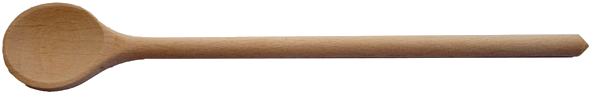
\includegraphics[width=\textwidth,height=1cm]{loeffel1}}\end{picture}}%E
\newcommand{\leftmarkfoot}{\begin{picture}(1,0)\put(0,0.05){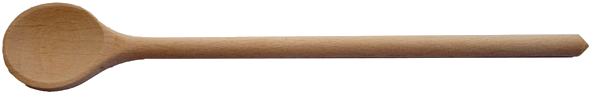
\includegraphics[width=\textwidth,height=1cm,angle=180]{loeffel1}}\end{picture}}%O
\usepackage[a4paper, margin=1in]{geometry}
\usepackage{authblk}
\setcounter{tocdepth}{2}
\usepackage{fancyhdr}
\pagestyle{fancy}
\renewcommand{\chaptermark}[1]{\markboth{#1}{}}
\renewcommand{\sectionmark}[1]{\markright{#1}{}}
\addtolength{\headheight}{2\baselineskip}
\fancyhf{}
%\fancyhead[EL]{\thepage}
\fancyhead[EC]{\thepage}
\fancyhead[ER]{\bfseries\rightmark}
\fancyhead[OL]{\bfseries\leftmark}
\fancyhead[OC]{\thepage}
%\fancyhead[OR]{\thepage}
\fancyfoot[ER]{\bfseries\rightmarkfoot}
\fancyfoot[OL]{\bfseries\leftmarkfoot}
\renewcommand{\headrulewidth}{.5pt}
\renewcommand{\footrulewidth}{.5pt}
\renewcommand{\headrulewidth}{0pt}
\renewcommand{\footrulewidth}{0pt}
\setlength{\unitlength}{\textheight} 
\addtolength{\unitlength}{\footskip} 
\addtolength{\unitlength}{\headsep} 
\addtolength{\unitlength}{2pt} 
%\renewcommand{\headrule}{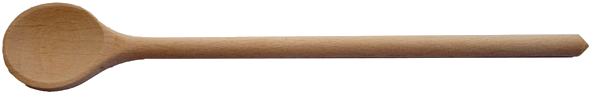
\includegraphics[width=\textwidth,height=2cm]{loeffel1}}
%\renewcommand{\footrule}{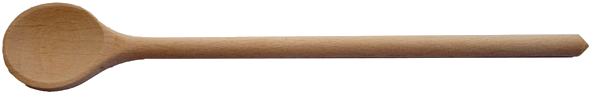
\includegraphics[width=\textwidth,height=2cm,angle=180]{loeffel1}}
\renewcommand{\leftmark}{\begin{picture}(1,0)\put(0,0.008){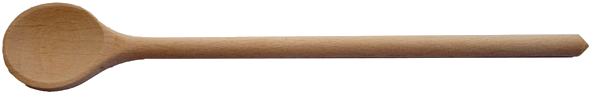
\includegraphics[width=\textwidth,height=1cm,angle=180]{loeffel1}}\end{picture}}%O
\renewcommand{\rightmark}{\begin{picture}(1,0)\put(0,-0.03){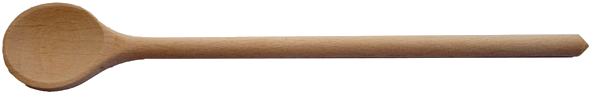
\includegraphics[width=\textwidth,height=1cm]{loeffel1}}\end{picture}}%E
%\renewcommand{\leftmark}{\begin{picture}(1,0)\put(-0.1,0.05){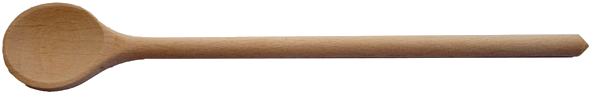
\includegraphics[width=1.2\textwidth,height=2cm,angle=180]{loeffel1}}\end{picture}}%O
%\renewcommand{\rightmark}{\begin{picture}(1,0)\put(-0.02,-0.025){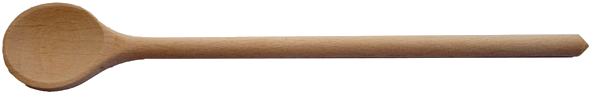
\includegraphics[width=1.2\textwidth,height=2cm]{loeffel1}}\end{picture}}%E
%on chapter and maketitle calls
\fancypagestyle{plain}{%
\fancyhead{}
\renewcommand{\headrulewidth}{0pt}
\renewcommand{\footrulewidth}{0pt}
\fancyfoot[OC]{\thepage}
\fancyfoot[EC]{\thepage}
}
\setlength{\topskip}{0mm}

\makeatletter
\def\thickhrulefill{\leavevmode \leaders \hrule height 1ex \hfill \kern \z@}
\def\@makechapterhead#1{%
  \vspace*{10\p@}%
  {\parindent \z@ \raggedleft \reset@font
            \scshape \@chapapp{} \thechapter
        \par\nobreak
        \interlinepenalty\@M
    \Huge \bfseries #1\par\nobreak
    %\vspace*{1\p@}%
    \hrulefill
    \par\nobreak
    \vskip 100\p@
  }}
\def\@makeschapterfoot#1{%
  \vspace*{10\p@}%
  {\parindent \z@ \raggedleft \reset@font
            \scshape \vphantom{\@chapapp{} \thechapter}
        \par\nobreak
        \interlinepenalty\@M
    \Huge \bfseries #1\par\nobreak
    %\vspace*{1\p@}%
    %\hrulefill
    \par\nobreak
    \vskip 100\p@
  }}
\makeatother



% configure recipe environment
\newcounter{stepcnt}

\newcommand{\preptime}[1]{\Interval\ #1\\[0.2cm]}
\newcommand{\person}[1]{\\\underline{\textit{Zutaten für #1 Person:}}\\[0.2cm]}
\newcommand{\persons}[1]{\\\underline{\textit{Zutaten für #1 Personen:}}\\[0.2cm]}
\newcommand{\portions}[1]{\\\underline{\textit{Zutaten für #1 Portionen:}}\\[0.2cm]}
\newcommand{\ingredientsec}[1]{\\\textbf{\textit{#1:}}\\[0.2cm]}
\newcommand{\ingredient}[1]{#1\\[0.2cm]}

\newcommand{\hour}{Stunde\xspace}
\newcommand{\hours}{Stunden\xspace}
\newcommand{\minute}{Minute\xspace}
\newcommand{\minutes}{Minuten\xspace}
\newcommand{\degree}{Grad\xspace}
\newcommand{\gramm}{$g$\xspace}
\newcommand{\liter}{$l$\xspace}
\newcommand{\cremefraiche}{Cr\`{e}me fra\^{i}che\xspace}

\newcommand{\recipe}[4]{
\newpage
\setcounter{stepcnt}{1}
\begin{tabularx}{\textwidth}{m{0.35\textwidth}m{0.65\textwidth}}
&\\
\centering
\includegraphics[width=0.3\textwidth]{#2}
&\section{#1}\\
\end{tabularx}
%
\vspace{0.5cm}
\rule{\textwidth}{1pt}
\vspace{0.5cm}
%
\begin{minipage}[t]{0.35\textwidth}
#3
\end{minipage}
%
\begin{minipage}[t]{0.65\textwidth}
\underline{\textit{Zubereitung:}}
\begin{list}{\textbf{\color{red}{\Large{\arabic{stepcnt}}}}}{\usecounter{stepcnt}\it}
#4
\end{list}
\end{minipage}
}




\usepackage[ % muss letztes Package sein!
	pdftitle={Mutti's Kochbuch},%
	pdfauthor={Hannelore Reinhart},%
	pdfsubject={Kochbuch},%
	pdfcreator={PDFLaTeX},
	pdfproducer={LaTeX mit Ubuntu},
	colorlinks=false, pdfborder={0 0 0}
]{hyperref} % 

\begin{document}
\dominitoc

% title page
\begin{titlepage}
\pagecolor{yellow} % auskommentieren für weissen Hintergrund
%\author{\copyright \ 2011 Hannelore Reinhart\\Layout: Felix Reinhart}
%\date{\today}
\title{\vspace{-4cm}
\Huge{\textbf{Mutti's Kochbuch}}
%\\\phantom{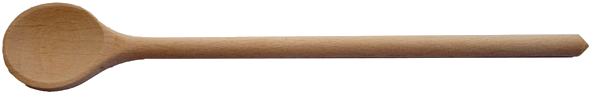
\includegraphics[width=15cm,angle=-90]{loeffel1}}
\begin{picture}(0.5,0.6)
\put(0.195,0.5){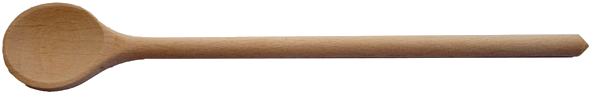
\includegraphics[width=20cm,angle=-90]{loeffel1}}
\put(0.163,0.32){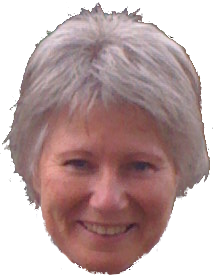
\includegraphics[height=6.5cm]{Mutti-head}}
\put(0,0.5){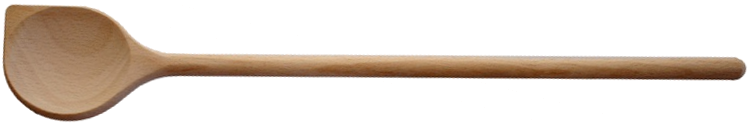
\includegraphics[width=20cm,angle=-90]{loeffel2}}
\put(0.39,0.5){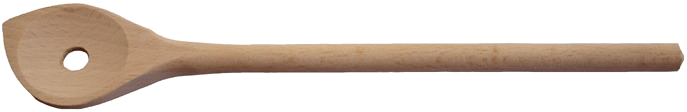
\includegraphics[width=20cm,angle=-90]{loeffel3}}
\end{picture}
}
\author{}
\date{}
\end{titlepage}
\maketitle
\pagecolor{white}
\pagestyle{empty}
%\cleardoublepage
\newpage

% copyright page
\begin{minipage}[b!]{\textwidth}
\begin{flushleft}
\flushbottom \copyright \ 2011 Hannelore Reinhart\\
Layout: Felix Reinhart\\
Datum: \date{\today}
\end{flushleft}
\end{minipage}

% table of contents
\setcounter{page}{1}
\tableofcontents
\pagestyle{fancy}
\cleardoublepage

%%%%%%%%%% Content %%%%%%%%%%%%%%%%%%%%%%%%%%%%%%%%%%%%%%%%%

\chapter{Suppen und Salate}
\minitoc
\recipe{{Grießklößchensuppe}}{Griesskloesschensuppe}{
\preptime{ca. 30 \minutes}
\persons{3--4}
\ingredient{50--60\gramm Butter}
\ingredient{1--2 Eier}
\ingredient{100--120\gramm Grieß}
\ingredient{Salz, Muskat, evtl. etwas \\ zerdrückten Knoblauch}
\ingredient{1$\frac{1}{2}$\liter Gemüsebrühe (instant)}
}{
\item Butter mit Schneebesen schaumig rühren, abwechselnd Grieß und Eier hinzugeben, würzen, Teig etwas anziehen lassen.
\item In die kochende Brühe mit nassem Kaffeelöffel (vorher in die heiße Brühe tauchen, damit der Teig sich besser vom Löffel löst) 
Klößchen einlegen und 10 bis 15 \minutes langsam ziehen lassen.
}

\recipe{{Bunter Salat}}{BunterSalat}{
\preptime{ca. 20--30 \minutes}
\persons{2}
\ingredient{Tomaten}
\ingredient{Paprikaschoten}
\ingredient{Gurke}
\ingredient{(rote) Zwiebel oder \\ Frühlingszwiebeln}
\ingredient{Mais aus der Dose}
\ingredient{Evtl. Blattsalat}
\ingredientsec{Weitere Zutaten}
\ingredient{Schafskäse}
\ingredient{Thunfisch aus der Dose}
\ingredient{Oliven}
\ingredient{In Olivenöl und Knoblauch gebratene Schrimps o.ä.}
\ingredientsec{Salatsoße}
\ingredient{1--2 Esslöffel Balsmico-\\Essig dunkel}
\ingredient{1 Esslöffel Olivenöl}
\ingredient{1 Prise Zucker}
\ingredient{1 Teelöffel gekörnte \\ (Gemüse-)Brühe}
\ingredient{Pfeffer}
\ingredient{Evtl. frische Kräuter \\ (z.B. Basilikum)}
}{
\item Aus den obigen Zutaten Salatsoße herstellen.
\item Gemüse waschen und klein schneiden nach Belieben.
\item Alles in die Salatschüssel geben und mit der Soße vermischen.
}

\recipe{{Tomaten mit Mozzarella}}{TomatenMozzarella}{
\preptime{ca. 15 \minutes}
\person{1}
\ingredient{2--3 Tomaten}
\ingredient{$\frac{1}{2}$ Päckchen Mozarella}
\ingredient{Balsamico-Essig dunkel}
\ingredient{Olivenöl}
\ingredient{Prise Zucker, Salz, Pfeffer}
\ingredient{Frisches Basilikum}
}{
\item Tomaten waschen und in Scheiben schneiden, auf einer Platte bzw. einem Teller anrichten. 
\item Salzen und pfeffern. 
\item Mozzarella in Scheiben schneiden und auf den Tomaten anrichten.
\item Aus Essig, Öl, Salz, Pfeffer und Zucker eine Soße herstellen und über die Tomaten und den Mozzarella verteilen.
\item Mit Basilikumblättern garnieren.
}


%\newpage
\chapter{Hauptgerichte}
\minitoc
\recipe{{Weißer Spargel}}{WeisserSpargel}{
\preptime{ca. $\frac{1}{2}$ \hour}
\persons{2}
\ingredient{1000\gramm weißer Spargel}
\ingredient{6--8 Frühlingskartoffeln \\ (je nach Größe}
\ingredient{6--8 Scheiben gekochter Schinken}
\ingredient{20--30\gramm Butter}
\ingredient{1 Knoblauchzehe}
\ingredient{Salz, Zucker, Muskat, Pfeffer, \\ frischer Thymian oder Rosmarin, 1~Teelöffel Zitronensaft}
}{
\item Kartoffeln waschen und in einem Sieb als Pellkartoffeln mit Thymian oder Rosmarin gar kochen.
\item Spargel schälen und waschen.
\item Kochwasser mit Zitronensaft, Salz, Zucker und Muskat den Spargel je nach Dicke der Stangen ca. 10--12 \minutes kochen, dann ausschalten und nach noch nachgaren. 
Die Stangen dürfen sich nicht zu sehr durchbiegen (Probe mit Messer machen).
\item In der Zwischenzeit die Butter im Stövchen mit zerdrückter Knoblauchzehe schmelzen und mit Salz und Pfeffer abschmecken.
\item Pellkartoffeln abpellen.
\item Spargel, Kartoffeln, Knoblauchbutter und Schinken anrichten.
\item Nach Belieben noch eine Sauce Hollandaise zubereiten. 
}

\recipe{{Pfannkuchen mit Spinat}}{PfannkuchenMitSpinat}{
\preptime{ca. 20--25 \minutes}
\persons{2}
\ingredient{250\gramm Mehl}
\ingredient{1 Ei}
\ingredient{Milch}
\ingredient{100\gramm Speckwürfel}
\ingredient{400\gramm Tiefkühlrahmspinat \\ (+ Blattspinat nach Belieben)}
\ingredient{Muskat, Salz, Pfeffer}
}{
\item Aus Mehl, Milch und Ei einen zähflüssigen Teig herstellen.
\item Den Tiefkühlspinat im Topf bei milder Hitze auftauen und mit Salz, Pfeffer und Muskat abschmecken.
\item Die Pfannkuchen im Fett mit den Speckwürfeln (1 mittlerer Esslöffel pro Pfannkuchen) ausbacken während der Spinat auftaut.
\item In der Zwischenzeit die Butter im Stövchen mit zerdrückter Knoblauchzehe schmelzen und mit Salz und Pfeffer abschmecken.
}

\recipe{{Pikanter Lauchkuchen \newline (oder Zucchinikuchen)}}{PikanterLauchkuchen}{
\preptime{Teig ca. 10 \minutes \\\phantom{\Interval} + 1 \hour Ruhezeit}
\preptime{Füllung 30 \minutes}
\preptime{Backzeit 25--30 \minutes}
\vspace{-0.3cm}
\persons{2--3}
\vspace{-0.4cm}
\ingredientsec{Teig}
\ingredient{200\gramm Mehl}
\ingredient{100\gramm kalte Magarine oder Butter}
\ingredient{1 Messerspitze Salz}
\ingredient{1--2 Esslöffel kaltes Wasser}
\ingredient{Öl zum Einfetten}
\ingredientsec{Lauchfüllung}
\ingredient{750\gramm Lauch}
\ingredient{100--125\gramm durchwachsener Speck}
\ingredient{2 Esslöffel Öl}
\ingredient{Etwas Zitronensaft}
\ingredient{Sojasoße, Pfeffer, Salz, Kümmel gemahlen, Muskat, süßes Paprikapulver}
\ingredient{1 Becher saure Sahne oder \\ \cremefraiche}
\ingredient{1--2 Eier}
\ingredient{50\gramm geriebener Käse (oder nach Belieben mehr)}
}{
\item Den Knetteig für eine Springform mit obigen Zutaten vorbereiten und kühl stellen.
\item Den Lauch putzen (waschen, gucken, dass kein Dreck mehr zwischen den einzelnen Schichten ist. 
Dafür u. U. die Lauchstangen der Länge nach halbieren und dann  waschen) und in kleine Stücke schneiden. 
\item Den Teig dünn ausrollen und kleinen Rand für die Springform herstellen. 
Mit der Gabel mehrmals einstechen und im Ofen bei ca. 200 Grad (Umluft 180 Grad) 10 \minutes vorbacken.
\item In der Zeit Speck und Lauch im Öl in einer Pfanne leicht andünsten und mit Zitronensaft, Sojasoße, Kümmel, Salz und Pfeffer abschmecken und etwas abkühlen lassen.
\item In dieser Zeit die Soße mit dem Mixer (Schneebesen) herstellen aus saurer Sahne, Ei und Gewürzen.
\item Auf dem vorgebackenen Boden Lauchfüllung verteilen und mit dem geriebenen Käse bestreuen.
\item Im Ofen bei 200 Grad (Umluft 180 Grad) ca. 25 \minutes backen.
%\setcounter{stepcnt}{-1}
\item Für die \textbf{Zucchinifüllung} die Zucchini waschen Ende abschneiden und in Scheiben schneiden. 
In Öl mit dem Speck anbraten und mit Zitronensaft, Sojasoße, Salz, Pfeffer abschmecken.
Für die Soße statt saurer Sahne süße Sahne verwenden oder auch \cremefraiche, sonst wie oben.
}

\recipe{{Blumenkohl-Nudel-Auflauf}}{Blumenkohlauflauf}{
\preptime{ca. 1 \hour}
\persons{2--3}
\ingredient{1 Blumenkohl}
\ingredient{250\gramm Nudeln oder Makkaroni}
\ingredient{Salzwasser für die Nudeln}
\ingredient{Salzwasser mit Muskat und etwas Milch für den Blumenkohl}
\ingredient{150\gramm Schinkenspeck}
\ingredient{2 Eier}
\ingredient{$\frac{1}{2}$ Becher \cremefraiche oder \\ süße Sahne}
\ingredient{1 Päckchen helle Soße \\ ($\frac{1}{4}$\liter Flüssigkeit)}
\ingredient{Zitronensaft, Muskat, Paprikapulver}
\ingredient{Geriebener Käse}
\ingredient{Öl oder Butter für die Auflaufform}
}{
\item Den Blumenkohl putzen, vom Strunk abtrennen, in Röschen zerteilen und waschen, abtropfen lassen. 
\item Das Wasser mit Salz und Muskat zum Kochen bringen, Milch hinzufügen (damit der Blumenkohl schön weiß bleibt). 
\item Dann die Blumenkohlröschen ins kochende Wasser legen und bei milder Hitze gar kochen (nicht zu weich!) und im Sieb abtropfen lassen.
\item Gleichzeitig auch das Nudelwasser zum Kochen bringen und die Nudeln nach Anleitung kochen und abschrecken, im Sieb abtropfen lassen.
\item Während der Kochzeit die Soße zubereiten. Dazu die helle Soße nach Anleitung zubereiten und mit Muskat und Zitronensaft abschmecken. 
\item Die Eier und die Sahne/\cremefraiche miteinander mit den Schneebesen verrühren und mit Paprikapulver leicht würzen. 
\item Beide Soßen miteinander vermischen, die helle Soße darf dabei nicht kochen!
\item Die Nudeln in die gefettete Auflaufform geben und mit den Speckwürfeln vermischen. 
\item Die Blumenkohlröschen auf den Nudeln verteilen und mit der Soße überziehen. 
\item Zuletzt den geriebenen Käse darüber geben.
\item Im Backofen bei 160--180 \degree 25--30 \minutes backen.
}

\recipe{{Lasagne mit Spinat und Lachs}}{LachsSpinatLasagne}{
\preptime{ca. 1 \hour}
\persons{2}
\ingredient{300\gramm Tiefkühlblattspinat}
\ingredient{8 Lasagneblätter \\ (ohne vorkochen)}
\ingredient{200--250\gramm Lachsfilet frisch \\ oder tiefgekühlt}
\ingredient{$\frac{1}{2}$\liter helle Soße (Päckchen)}
\ingredient{150\gramm geriebener Käse}
\ingredient{Öl, Salz, Pfeffer, Muskat, Zitronensaft, Knoblauchzehe, evtl. Zwiebel}
}{
\item Lachsfilet (auftauen), waschen, säuern, salzen und ziehen lassen. 
\item Tiefkühlspinat auftauen (Mikrowelle oder im Topf in kochendem Salzwasser).
\item Abgetropften Spinat in heißem Öl mit klein geschnittenem Knoblauch (evtl. mit Zwiebelwürfeln) andünsten und mit Salz, Pfeffer und Muskat abschmecken. 
\item Die helle Soße nach Anleitung zubereiten.
\item Den Fisch in kleine Stücke schneiden.
\item Die Auflaufform mit Öl auspinseln. 
\item Lagenweise die Lasagneblätter, Soße, Spinat, Soße, Fisch, Lasagneblätter, Soße, Spinat, Soße, Spinat und Käse in die Auflaufform füllen.
\item Die Lasagne im Backofen bei 200 \degree (Umluft 170 \degree) 25--30 \minutes backen.
}

\recipe{{Forelle in Alufolie}}{ForelleAlufolie}{
\preptime{ca. 45 \minutes}
\persons{2}
\ingredient{2 mittelgroße, ausgenommene \\ Forellen}
\ingredient{1 Strauß glatte Petersilie}
\ingredient{1--2 Knoblauchzehen}
\ingredient{2 Zitronenviertel}
\ingredient{Salz, Pfeffer, Zitronensaft, Öl}
\ingredient{Alufolie}
}{
\item Forellen waschen, mit Zitronensaft den Bauchraum auströpfeln, salzen, pfeffern und ziehen lassen.
\item Petersilie waschen, Knoblauch schälen und in kleine Scheiben schneiden. Petersilie und Knoblauchscheiben in den Bauch füllen.
\item Alufolie in Stücke trennen und mit Öl bepinseln.
\item Die vorbereiteten Forellen in die Mitte legen und die Folie zusammenrollen und -drücken.
\item Im Backofen bei 200 \degree 20--25 \minutes backen.
\item Mit Zitronenvierteln servieren.
\item Als \textbf{Beilagen} reicht man Salz- oder Pellkartoffeln mit gekochtem Gemüse (Möhren, Broccoli o.a.) oder grünen Salat.
\item \textbf{Variation mit Mandelbutter:} In heißer Butter in einer Pfanne Mandelblättchen sanft bräunen und zur Forelle reichen.
}

\recipe{{Sauerkraut mit Flönz und Kartoffelpüree}}{Sauerkraut2}{
\preptime{ca. 45 \minutes}
\persons{2--4}
\ingredient{1 Dose Mildessa Sauerkraut \\ (oder anderes)}
\ingredient{1 große Zwiebel}
\ingredient{1 Apfel}
\ingredient{Öl oder Schmalz}
\ingredient{Etwas Speckwürfel}
\ingredient{1--2 Lorbeerblätter}
\ingredient{ca. 4 Wacholderbeeren}
\ingredient{1 Teelöffel Kümmel}
\ingredient{$\frac{1}{4}$\liter Gemüsebrühe (instant)}
\ingredient{1 Esslöffel Honig}
\ingredient{Pfeffer}
\ingredient{$\frac{1}{2}$--1 Ring geräucherte Blutwurst}% \\ im Naturdarm}
\ingredient{Mehl zum Stäuben}
\ingredient{Senf}
\ingredient{Kartoffeln, Salz, Milch, Muskat}
}{
\item Kartoffeln schälen und in Würfel schneiden.
\item Salzkartoffeln kochen.
\item Für das Sauerkraut die Zwiebel und den Apfel klein schneiden. 
\item Öl oder Schmalz erhitzen und Zwiebeln, Speckwürfel und Apfel andünsten. 
\item Das Sauerkraut dazugeben und mit der Brühe ablöschen. 
\item Gewürze dazu geben und 15 \minutes köcheln lassen. Mit Honig abschmecken.
\item Das Püree aus den fertig gekochten Salzkartoffeln zubereiten. Kartoffeln abgießen und mit etwas Milch im Topf erwärmen. 
\item Mit den Schneebesen und dem Mixer alles in einem Rührbecher zusammen mit Muskat und Salz schlagen. Evtl. noch Milch hinzufügen, falls das Püree zu fest ist.
\item In einer Pfanne das Öl erhitzen und die in Scheiben geschnittene und mit Mehl bestäubte Flönz von beiden Seiten kurz und sanft braten.
\item Als \textbf{Variation} auch Nürnberger Rostbratwürstchen oder Leberkäse im Kraut erwärmen oder separat braten.
\item Zu den Fleischbeilagen Senf reichen.
}


%\newpage
\chapter{Desserts und Süßspeisen}
\minitoc
\recipe{Tiramisu}{Tiramisu}{
\preptime{ca. $\frac{1}{2}$ \hour}
\portions{8}%\persons{8}
\ingredient{500\gramm Löffelbisquits}
\ingredient{500\gramm Mascapone}
\ingredient{4 Eier}
\ingredient{125\gramm Zucker}
\ingredient{10 Esslöffel Amaretto}
\ingredient{1 Tasse starken Kaffee \\ (mit Zucker)}
\ingredient{10\gramm (1 Esslöffel) Pudergelantine}
\ingredient{Kakaopulver}
}{
\item Kaffee kochen, süßen und abkühlen lassen.
\item Eier trennen.
\item Eiweiß steif schlagen.
\item Eigelb und Zucker cremig rühren.
\item Mascapone, Pudergelantine und Amaretto dazugeben.
\item Eiweiß unter die Creme heben.
\item Löffelbisquits mit Kaffee beträufeln \\ (ca. 1 Teelöffel pro Bisquit).
\item Bisquits und Creme in Schale schichten \\ (Bisquit, Creme, Bisquit, Creme).
\item 3 Stunden kalt stellen.
\item Vor dem Verzehr mit Kakaopulver bestreuen.
}

\recipe{Kaiserschmarrn}{KaiserschmarrnPreiselbeeren}{
\preptime{ca. 20 \minutes}
\persons{1}
\ingredient{125\gramm Mehl}
\ingredient{4 Eier}
\ingredient{$\frac{1}{4}$\liter Milch}
\ingredient{1 Prise Salz}
\ingredient{Sultaninen}
\ingredient{Butter zum Ausbacken}
\ingredient{Puderzucker zum Bestreuen}
\ingredient{Obstkonserve oder als Kompott frisch z.B. Glas Kirschen vom Vater oder Apfelmus}
}{
\item Eier trennen und das Eiklar zu Schnee schlagen.
\item Mehl, Eigelb, Milch, Salz mit den Schneebesen zu einem glatten Teig verrühren. Den Eischnee darunter heben.
\item Butter in einer Pfanne erhitzen und den Teig hinein geben. Die Sultaninen dazugeben und alles bei milder Hitze backen. 
\item Wenn die zweite Seite gebacken ist, mit einem Pfannenwender alles zerstoßen und nochmals kurz rösten. 
\item Mit Puderzucker bestreuen.
\item Dazu reicht man das Kompott.
}

\recipe{{Grießbrei mit Obst}}{GriessbreiObst}{
\preptime{ca. 20 \minutes}
\persons{1--2}
\ingredient{1\liter Milch}
\ingredient{4 Esslöffel Zucker}
\ingredient{1 Prise Salz}
\ingredient{Zitronenschale}
\ingredient{125--130\gramm Grieß (Hartweizen oder Weichweizen)}
\ingredient{2 haselnussgroße Stückchen \\ Butter}
\ingredient{Evtl. 1 Ei}
\ingredient{Obst}
}{
\item Milch mit Zucker zum Kochen bringen, Salz und Zitronenschale hinzugeben.
\item Von der Herdplatte nehmen und den Grieß reinrieseln lassen. Mit einem Schneebesen umrühren und auf der ausgeschalteten Herdplatte ca. 10--15 \minutes quellen lassen.
\item Die Butter dazu geben und evtl. ein Ei ganz oder nur das Eigelb einrühren.
\item Frisches Obst (Erdbeeren), frischen Kompott oder Obst aus der Konserve (z.B. vom Vater) dazu reichen.
\item \textbf{Alternativ mit Milchreis:} 1\liter Milch mit Zucker zum Kochen bringen. 200\gramm Milchreis in die kochende Milch geben. Zitronenschale und Prise Salz dazu geben, umrühren.
Die Masse bei ganz geringer Temperatur 30--45 \minutes ausquellen lassen. Aufpassen, dass der Reis nicht anliegt bzw. überkocht. Zwischendurch umrühren. Zubereitungszeit: ca. 50 \minutes. 
}

\recipe{Schneetorte}{Schneetorte}{
\preptime{Böden 30--50 \minutes je \\\phantom{\Interval} nach Anzahl der Backformen}
\preptime{Füllung 20 \minutes}
\preptime{Kühlzeit mindestens \\\phantom{\Interval} 1$\frac{1}{2}$--2 \hours}
\vspace{-0.3cm}
\portions{16}
\vspace{-0.4cm}
\ingredientsec{Teig}
\ingredient{100\gramm Margarine}
\ingredient{100\gramm Zucker}
\ingredient{1 Päckchen Vanillezucker}
\ingredient{1 Prise Salz}
\ingredient{4 Eigelbe}
\ingredient{125\gramm Mehl}
\ingredient{$\frac{1}{2}$ Teelöffel Backpulver}
\vspace{-0.4cm}
\ingredientsec{Belag}
\ingredient{4 Eiweiß}
\ingredient{200\gramm Zucker}
\ingredient{100\gramm gehobelte Mandeln}
\vspace{-0.4cm}
\ingredientsec{Füllung}
\ingredient{375--500\gramm Obst \\ (z.B. Beeren, Pfirsiche o.ä.)}
\ingredient{1--2 Päckchen Tortenguss, Zucker}
\ingredient{1--2 Becher Schlagsahne}
\ingredient{2 Päckchen Sahnesteif}
\ingredient{Evtl. statt dem 2. Becher Sahne 1 Becher Joghurt, dann etwas Gelatine (instant)}
\ingredient{Zucker}
}{
\item Die Eier trennen und das Eiklar steif schlagen und den Zucker unterschlagen.
\item Aus Margarine, Zucker, Eigelb, Vanillezucker, Salz, Mehl und Backpulver einen Rührteig herstellen.
\item Den Teig in zwei gleichgroße Teile teilen und in 2 gleichgroßen Springformen oder nacheinander in eine Springform geben.
\item Eine Hälfte des Eischnees auf dem Teig verteilen und die Hälfte der Mandeln darüber geben.
\item Im Backofen beide Böden bei 175--200 \degree 20 \minutes backen.
\item Die Ränder vorsichtig lösen und erkalten lassen.
\item Je nach dem im Anschluss dann den 2. Boden backen.
\item Wenn alles erkaltet ist, die Füllung auf den unteren Boden aufbringen. 
\item \textbf{Zubereitung der Füllung:}
\begin{enumerate}
\item Gut abgetropfte Früchte auf dem Boden verteilen. 
\item Tortenguss mit Wasser oder Fruchtsaft und Zucker herstellen und über die Früchte geben. 
\item Die Sahne mit Zucker steif schlagen, Sahnesteif nach Anweisung dazu geben (evtl. vorher den Joghurt mit Zucker verrühren und die Sahne darunter heben). 
\end{enumerate}
\item Die Masse über den Früchten gleichmäßig verteilen und den zweiten Boden draufsetzen.
\item Die Torte im Kühlschrank aufbewahren.
}

\recipe{Schokoladenkuchen}{Schokoladenkuchen}{
\preptime{ca. $\frac{3}{4}$ \hour}
%\portions{8}
\persons{8}
\ingredient{250\gramm Margarine}
\ingredient{350\gramm Zucker}
\ingredient{350\gramm Mehl}
\ingredient{4 Eier}
\ingredient{4 Esslöffel Kakao}
\ingredient{1 Päckchen Backpulver}
\ingredient{1/2 Glass Wasser}
}{
\item Magarine in Topf schmelzen.
\item Schrittweise Zucker, Kakao und Wasser unter Rühren hinzufügen und gesamte Masse zum Kochen bringen.
\item 1/2 Glass der Kakaomasse für späteren Guss abfüllen.
\item Eier, Mehl und Backpulver mit Kakaomasse anrühren.
\item Kuchenform einfetten und mit Paniermehl einstäuben. Kuchenmasse einfüllen.
\item Kuchen im vorgeheizten Ofen bei 175 \degree ca. 45 \minutes backen.
\item Kuchen vor dem Stürzen aus der Form ca. 1 Stunde abkühlen lassen.
\item Kuchen mit dem Guss besteichen. Wenn der Guss zu kühl ist, kurz in der Mikrowelle bei 300 Watt für ca. 30 Sekunden aufwärmen.
\item Guss abkühlen lassen.
}



%%%%%%%%%%%%%%%%%%%%%%%%%%%%%%%%%%%%%%%%%%%%%%%%%%%%%%%%%%%%%

% finish
\cleardoublepage
\pagestyle{empty}
\cleardoublepage
\newpage
\phantom{blub}
\newpage
\pagecolor{yellow} % auskommentieren für weissen Hintergrund

% rear page
\begin{center}
\begin{picture}(0,0)
\put(-0.07,-0.07){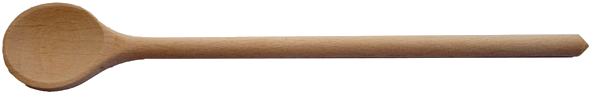
\includegraphics[width=20cm,angle=-110]{loeffel1}}
\put(-0.31,-0.11){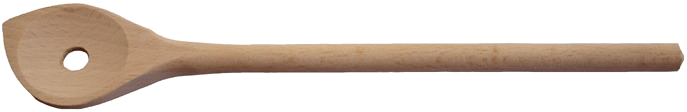
\includegraphics[width=20cm,angle=-70]{loeffel3}}
\put(-0.06,-0.05){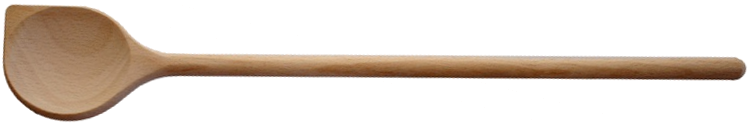
\includegraphics[width=20cm,angle=-90]{loeffel2}}
\end{picture}
\end{center}

\end{document}

